\section{WIP: Implementation Note of PEG Parser}

\subsubsection{Normalizing}

\begin{align*}
  \begin{array}{rclr}
  e_{\mathrm{RHS}}
  & \Coloneq & e_1 \mathrel{/} \cdots \mathrel{/} e_n \mathrel{/} \epsilon &(n \in \Natural) \\
  & \mid & e_1 \mathrel{/} \cdots \mathrel{/} e_n &(n \in \Natural_{\geq 1}) \\
  e
  & \Coloneq & \mathop{!} (u_1 \cdots u_n) &(n \in \Natural_{\geq 1}) \\
  & \mid & \mathop{\&} (u_1 \cdots u_n) &(n \in \Natural_{\geq 1}) \\
  & \mid & u_1 \cdots u_n &(n \in \Natural_{\geq 1}) \\
  u
  & \Coloneq & \sigma \\
  & \mid & A
  \end{array}
\end{align*}

\begin{align*}
  \symnorm(N, []) &= (N, \emptyset) \\
  \symnorm(N, [A \assign e] + X) &= (N_2, \{A \assign \symalt(a)\} \cup X_1 \cup X_2) \\
  &\hspace{3em}(\symnorm(N, e) = (a, N_1, X_1), \symnorm(N_1, X) = (N_2, X_2))
\end{align*}

\begin{align*}
  \symnorm(N, \epsilon) &= ([\epsilon], N, \emptyset) \\
  \symnorm(N, \sigma) &= ([\sigma], N, \emptyset) \\
  \symnorm(N, A) &= ([A], N, \emptyset) \\
  \symnorm(N, e_1 e_2) &= (\symseq(a_1, a_2), N_2, X_1 \cup X_2) &(\symnorm(N, e_1) = (a_1, N_1, X_1), \symnorm(N_1, e_2) = (a_2, N_2, X_2)) \\
  \symnorm(N, e_1 / e_2) &= (a_1 + a_2, N_2, X_1 \cup X_2) &(\symnorm(N, e_1) = (a_1, N_1, X_1), \symnorm(N_1, e_2) = (a_2, N_2, X_2)) \\
  \symnorm(N, e^*) &= ([M], N' \uplus \{M\}, X \cup \{M \assign A M / \epsilon\}) &(\symnorm(N \uplus \{A\}, [A \assign e]) = (N', X)) \\
  \symnorm(N, \mathop{\&} e) &= ([M], N' \uplus \{M\}, X \cup \{M \assign \mathop{\&} A\}) &(\symnorm(N \plus \{A\}, [A \assign e]) = (N', X)) \\
  \symnorm(N, \mathop{!} e) &= ([M], N' \uplus \{M\}, X \cup \{M \assign \mathop{!} A\}) &(\symnorm(N \plus \{A\}, [A \assign e]) = (N', X))
\end{align*}

\begin{align*}
  \symseq(a_1, a_2) &= [e_1 e_2 \mid e_1 \assign a_1, e_2 \assign a_2] \\
  \symalt([e_1, \ldots, e_n]) &= e_1 / \cdots / e_m &(\forall i < m\ldotp e_i \neq \epsilon, e_m = \epsilon) \\
  \symalt([e_1, \ldots, e_n]) &= e_1 / \cdots / e_n &(\forall i\ldotp e_i \neq \epsilon)
\end{align*}

\begin{gather*}
  \symnorm((\Sigma, N, R, e_0)) = (\Sigma, N', R', S) \\
  (R = \{A_1 \assign e_1, \ldots, A_n \assign e_n\}, \symnorm(N \uplus \{S\}, [S \assign e_0, A_1 \assign e_1, \ldots, A_n \assign e_n]) = (N', R'))
\end{gather*}

\subsubsection{Machine}

State:
\begin{itemize}
  \item a rule
  \item current position in rule
\end{itemize}

Transition:
\begin{itemize}
  \item $\sigma$
  \item EOS
  \item otherwise
\end{itemize}

Output:
\begin{description}
  \item[with backpoint] バックポイントを設置し,バックポイントに戻った時の次の遷移を指定する.fail した場合一番直近の backpoint まで入力状態とスタックを戻す.reduce 時取り除かれる.
  \item[enter] 非終端記号を参照する.メモ化されている場合その値を使う.それ以外の場合,reduce 時戻ってくる状態を記録し,次の状態に遷移する.
  \item[goto] 次の状態に遷移する.
  \item[shift] 入力を1つ消費し,次の状態に遷移する.
  \item[reduce] 規則に沿ってスタックから要素を取り出してまとめ,メモし,スタックに新たに入れた後,enter 時に記録された状態に遷移する.
\end{description}

\subsubsection{Optimization}

\begin{enumerate}
  \item unify transitions.
  \item look ahead backpoints.
\end{enumerate}

\subsubsection{Example}

\begin{align*}
  \begin{array}{rcl}
  E
  & \Coloneq & C A \\
  & \mid & \epsilon \\
  A
  & \Coloneq & a B \\
  & \mid & a \\
  B
  & \Coloneq & b A \\
  & \mid & b \\
  C
  & \Coloneq & \mathop{!} abab \\
  & \mid & \mathop{\&} ab
  \end{array}
\end{align*}

\begin{figure}
  \centering
  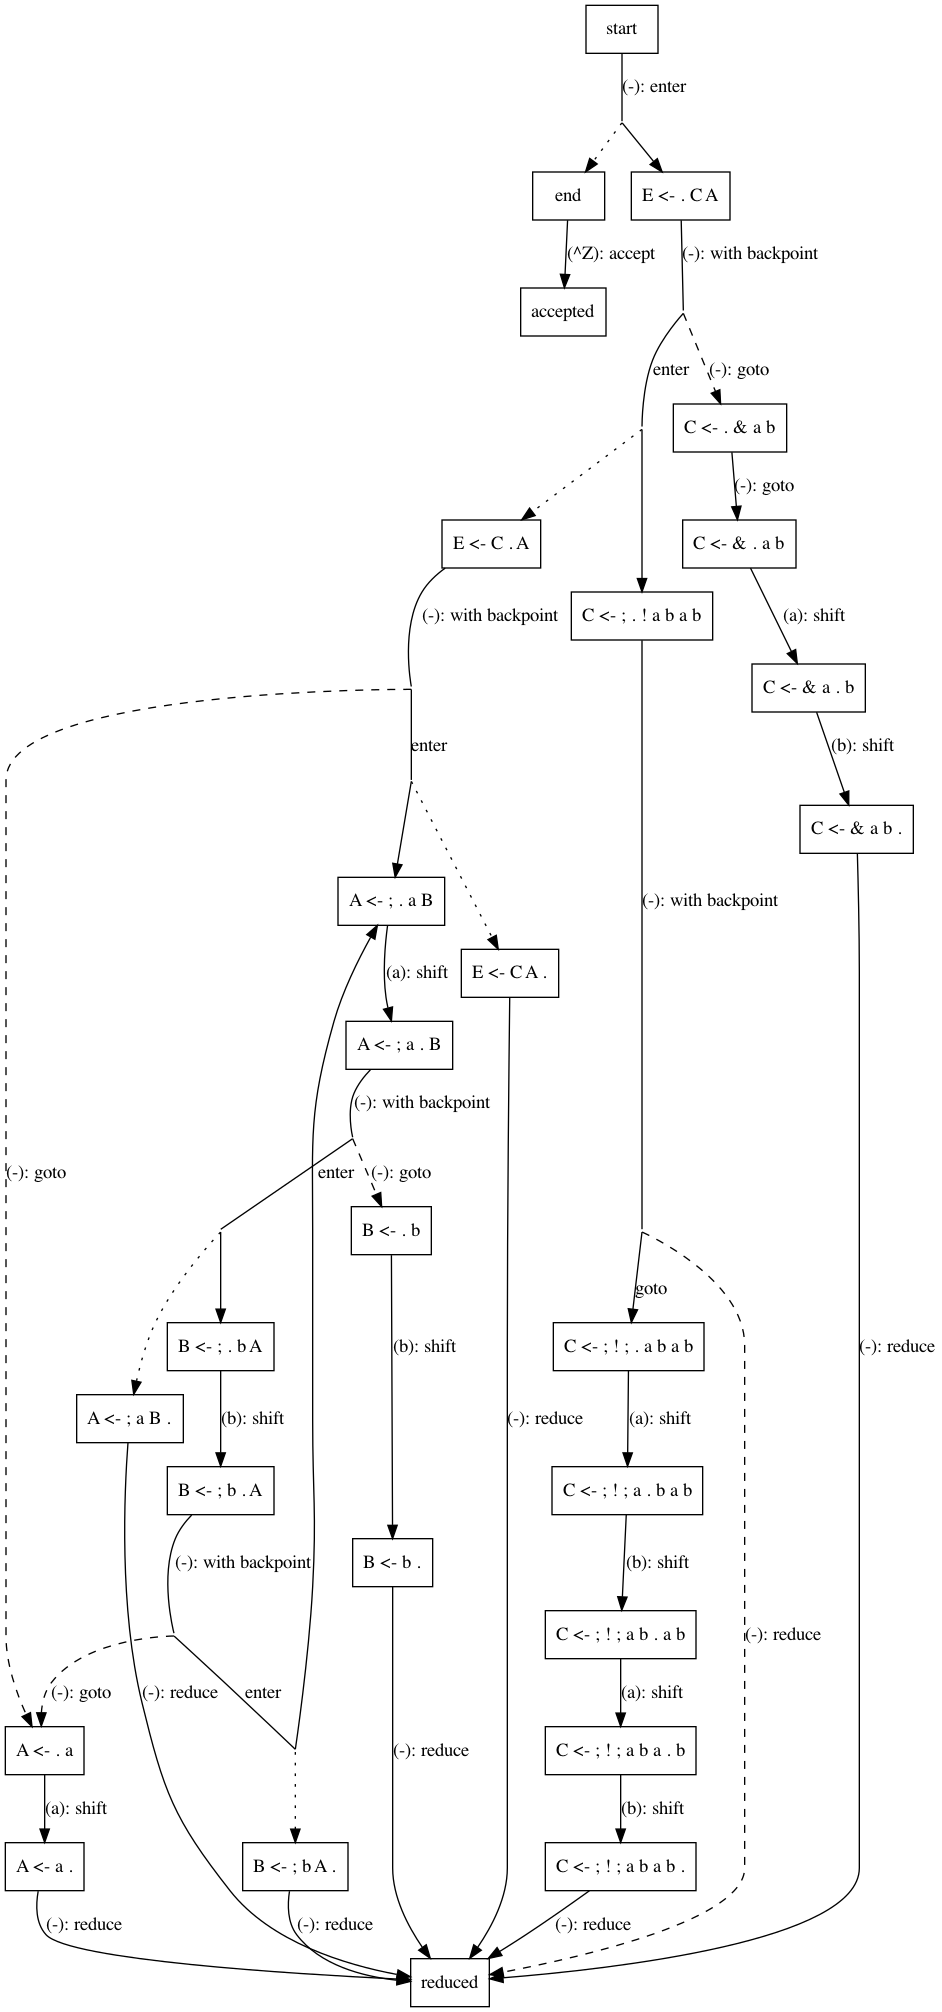
\includegraphics[height=0.9\textheight]{asset/implementation-note-of-peg-parser/sample-grammar.png}
  \caption{状態遷移図}
  \label{implementation-note-of-peg-parser:figure:example}
\end{figure}

\begin{figure}
  \centering
  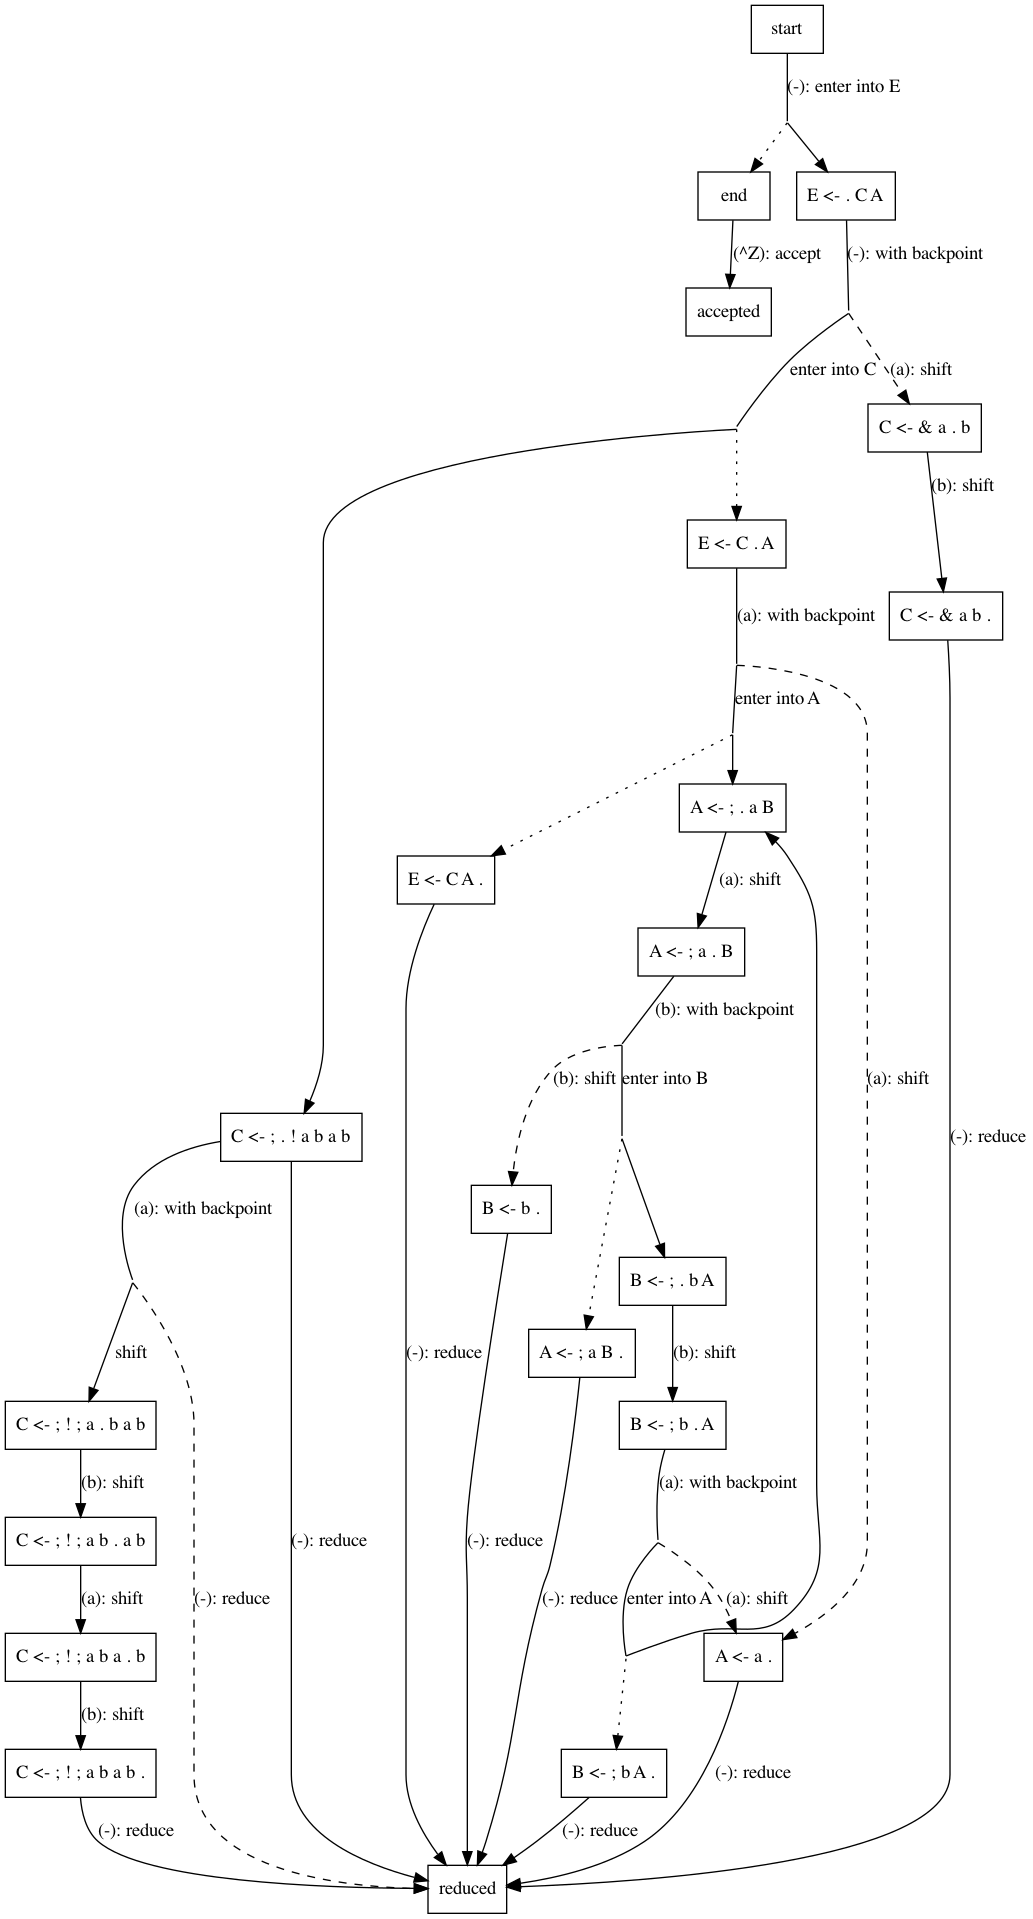
\includegraphics[height=0.9\textheight]{asset/implementation-note-of-peg-parser/sample-grammar-optimized.png}
  \caption{最適化された状態遷移図}
  \label{implementation-note-of-peg-parser:figure:example-optimized}
\end{figure}
